\documentclass{article}
\usepackage{graphicx}

\title{E14 Meeting}
\author{Toby Bourke}
\date{May 3rd 2021}
\usepackage[a4paper, margin=4cm]{geometry}

\begin{document}

\begin{titlepage}
\maketitle
\end{titlepage}

\section{Signal Start Detection}
\subsection{The Problem}
To find the start of a signal that has been emitted from another device isn't a simple problem to solve. This is because sound can ramp up when initially transmitted. Due to this ramp up, the start can be hard to find as the signal needs to be clear to detect it.

\subsection{The Different Approaches}
The different possible approaches to finding the start point of the signal are as follows:

\begin{itemize}
\item Audio Onset Detection
\item Anomaly Detection/Outlier Detection
\end{itemize}

These approaches are really more categories of approaches than actually approaches themselves.\\

Audio Onset Detection is focused primarily on sound and detecting when a sound/note/frequency starts. Within this category of detection, there are an incredibly large amount of approaches ranging from Neural Networks to simple amplitude detection.\\

Anomaly Detection is also a category like Audio Onset Detection, and has many approaches to achieve the similar things. This approach is different to Audio Onset Detection as its meant for anomalies in data and not specifically audio. It has a similarly expansive detection method to Audio Onset ranging from Neural Networks to Density-based techniques.

Between Audio Onset and Anomaly Detection there overlap as they are more or less achieving similar things for different tasks. Due to how extreme the overlap is, Audio Onset was the only one further researched as its more fit for task.

\subsubsection{Audio Onset Detection}
There are endless approaches to Audio Onset Detection (AOD) that have been developed, so to determine which is best fit for purpose is difficult. As AOD gets more accurate, the processing power increases significantly.\\

\begin{figure}
	\centering
	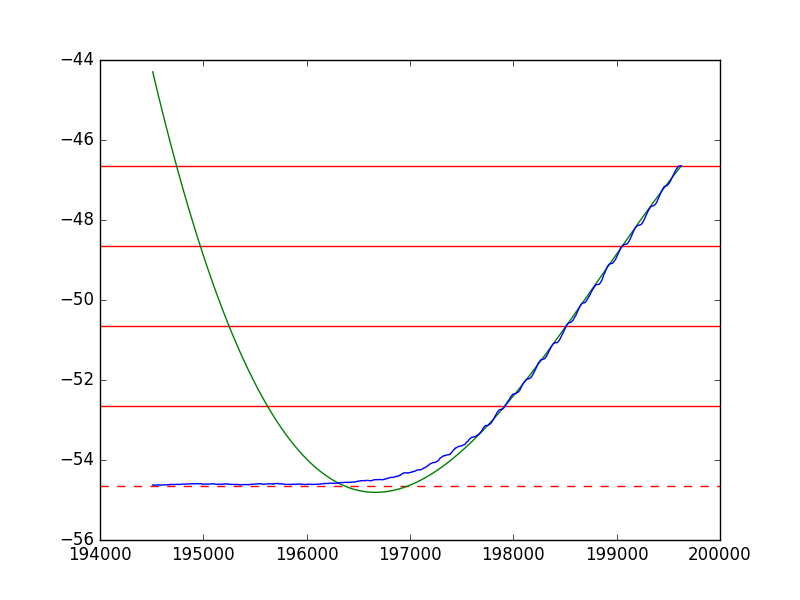
\includegraphics[width=10cm]{signalShapeOverlay}
	\caption{An input signal being overlapped with know shape}
	\label{fig:signalShapeOverlay}
\end{figure}

A simple form of AOD of a known signal shape is by overlapping the expect shape of the input signal over the actual signal. By overlapping these two, the start location of the signal can be found. An example of this can be seen in Figure \ref{fig:signalShapeOverlay}.\\

\begin{figure}
	\centering
	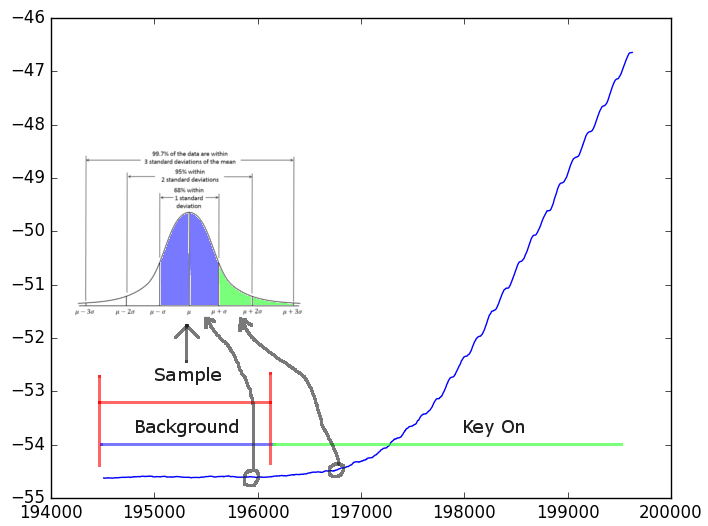
\includegraphics[width=10cm]{signalProbablity}
	\caption{Probability of each point on a signal being noise or known signal.}
	\label{fig:signalProb}
\end{figure}

Another form of AOD is shown in Figure \ref{fig:signalProb}. This form of AOD uses probability to detect when a signal starts, this can be effective with signals that aren't always what is expected.

\subsection{Experimentation}
Initial experimentation with recording and displaying sound was done to help prepare for use of actual hardware. This initial experimentation was done using a laptop mic and a phone emitting a tone. Due to the limitations of this setup, preliminary distance measurements are not easy to achieve.

In the figures below is data shown for multiple different test cases.

\begin{figure}
	\centering
	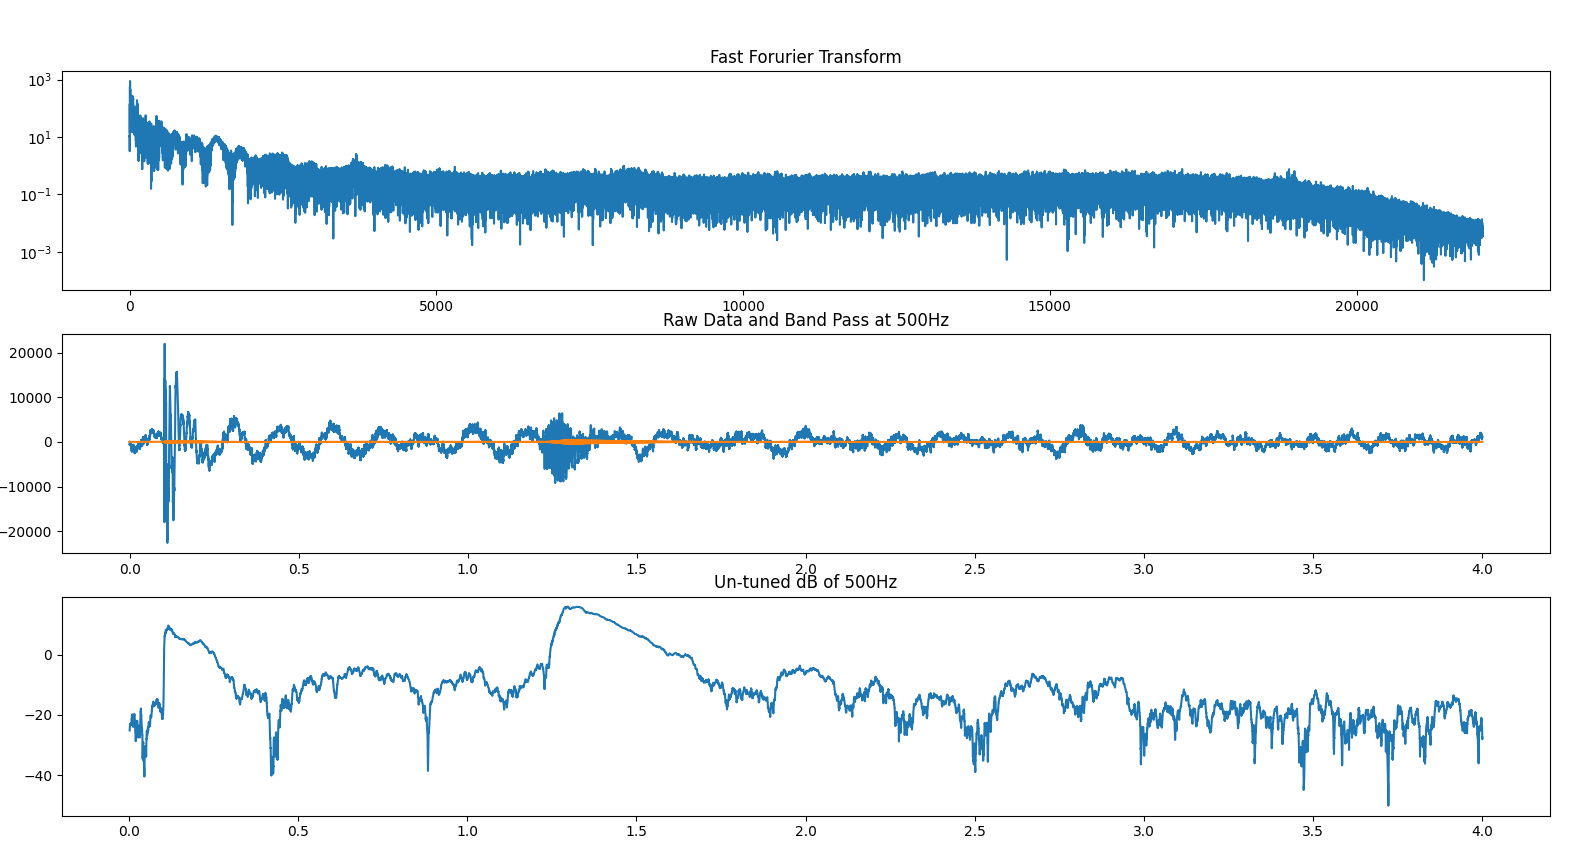
\includegraphics[width=10cm]{BackgroundNoise}
	\caption{Background noise of uncontrolled test environment}
	\label{fig:signalShapeOverlay}
\end{figure}

\begin{figure}
	\centering
	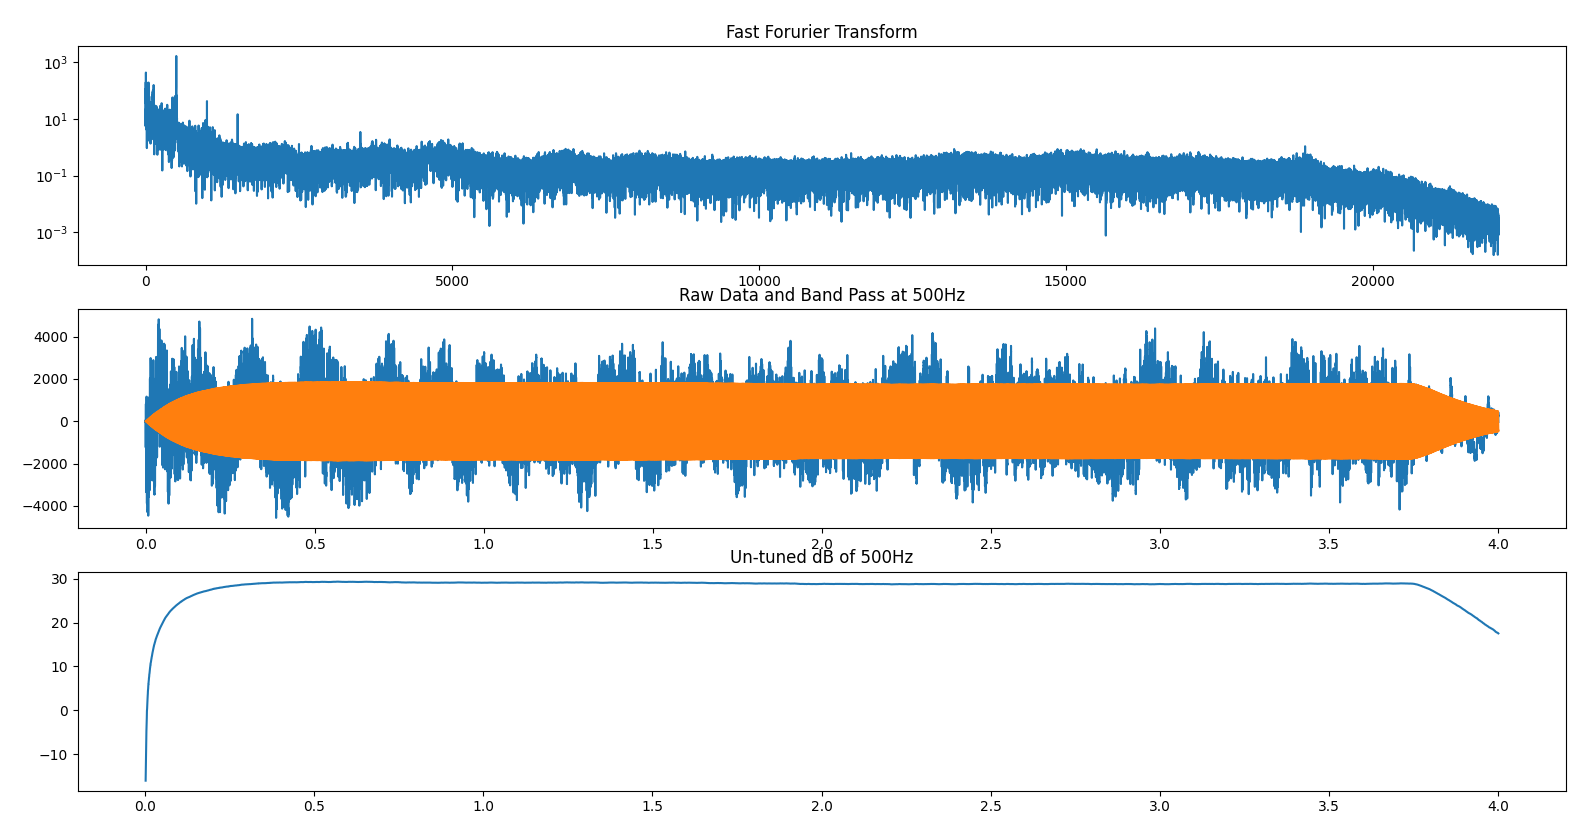
\includegraphics[width=10cm]{MostlyConstant500Hz}
	\caption{A 500Hz tone being played for most of the recorded 4 second time}
	\label{fig:signalShapeOverlay}
\end{figure}

\begin{figure}
	\centering
	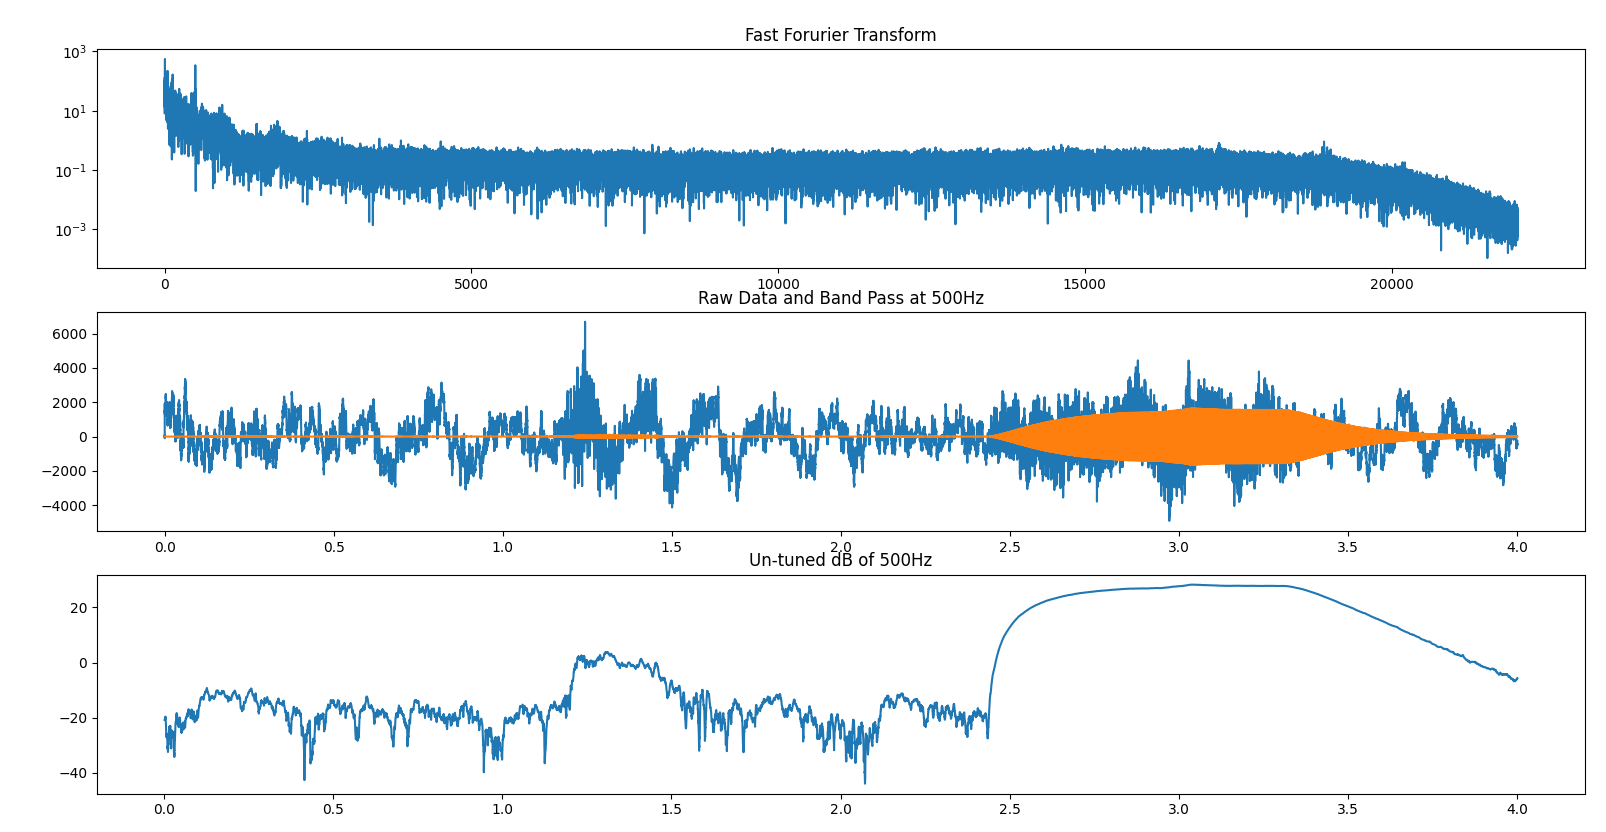
\includegraphics[width=10cm]{Pulse500Hz}
	\caption{A 500Hz tone being pulsed for a short period}
	\label{fig:signalShapeOverlay}
\end{figure}

\begin{figure}
	\centering
	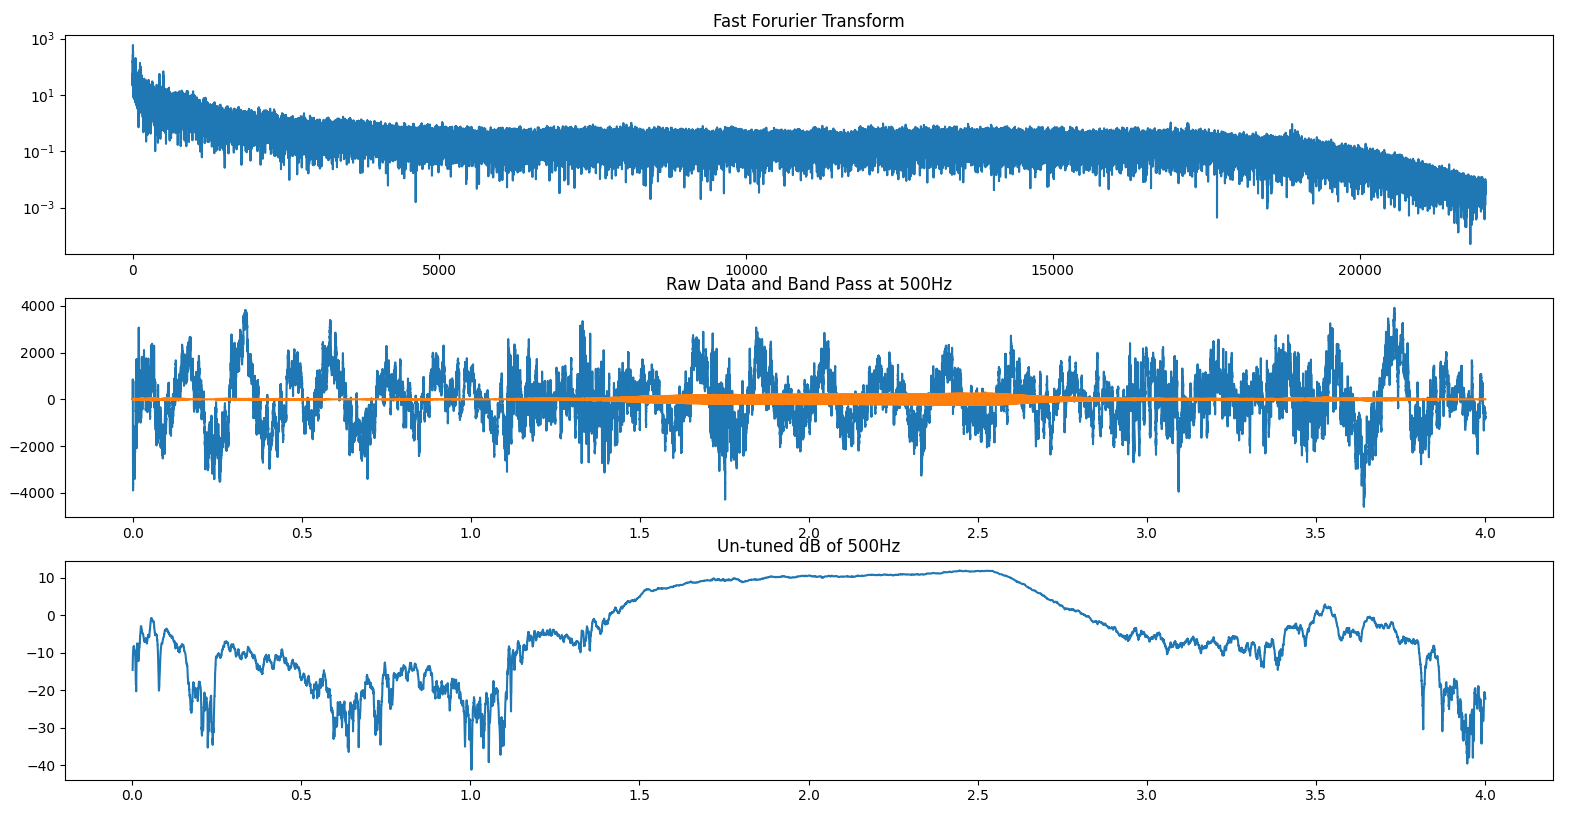
\includegraphics[width=10cm]{pulse500HzFar}
	\caption{A 500Hz tone being pulsed for a short period}
	\label{fig:signalShapeOverlay}
\end{figure}

\begin{figure}
	\centering
	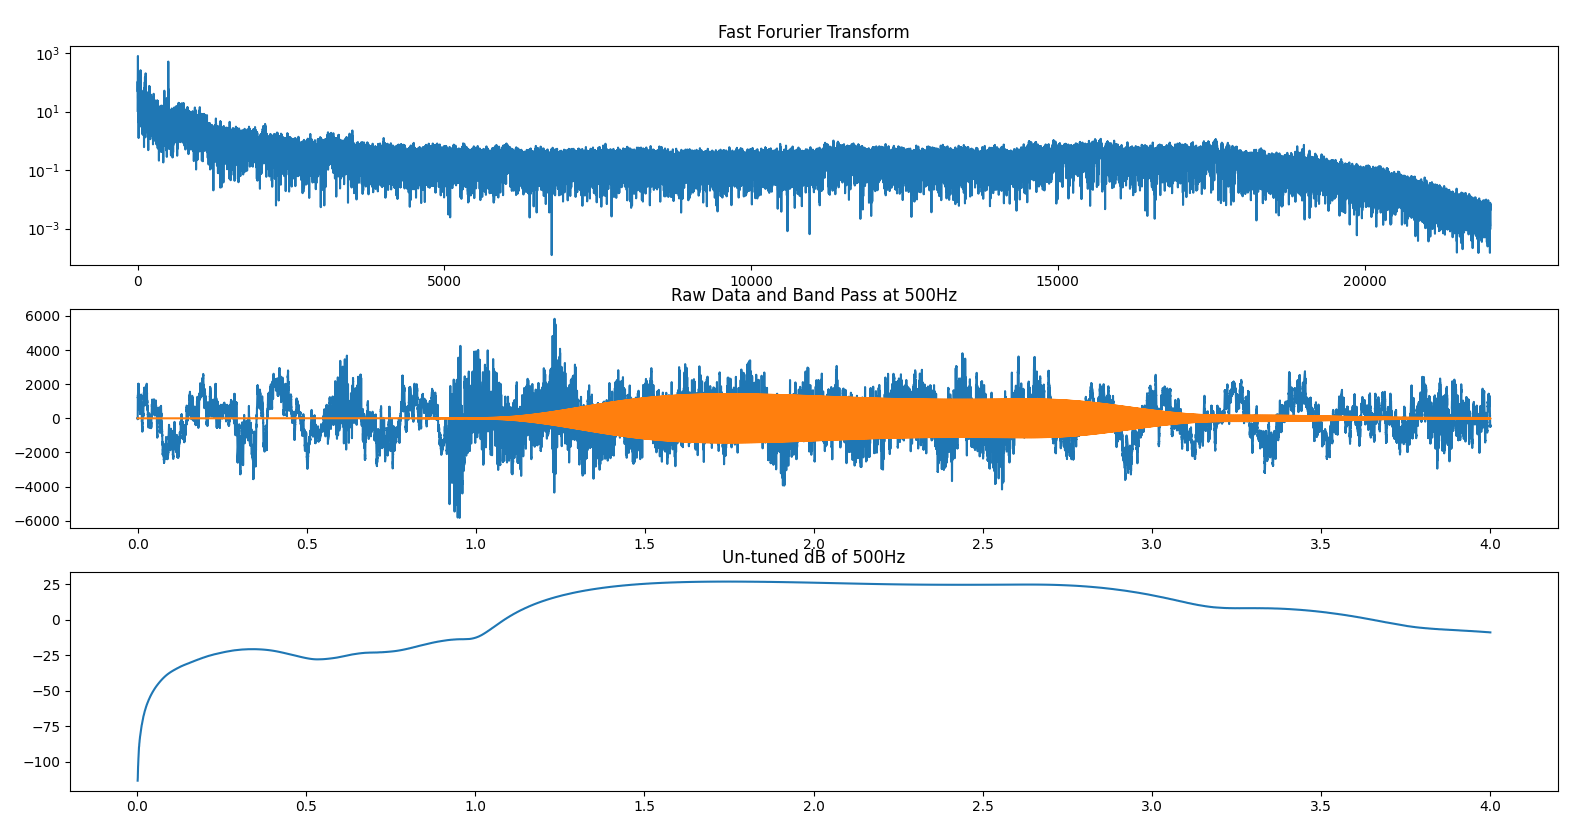
\includegraphics[width=10cm]{500Hz3order}
	\caption{A 500Hz tone being pulsed for a short period with 3rd Order Filter}
	\label{fig:signalShapeOverlay}
\end{figure}

\end{document}